\documentclass{article}
\usepackage{preamble}

\begin{document}

\begin{center}
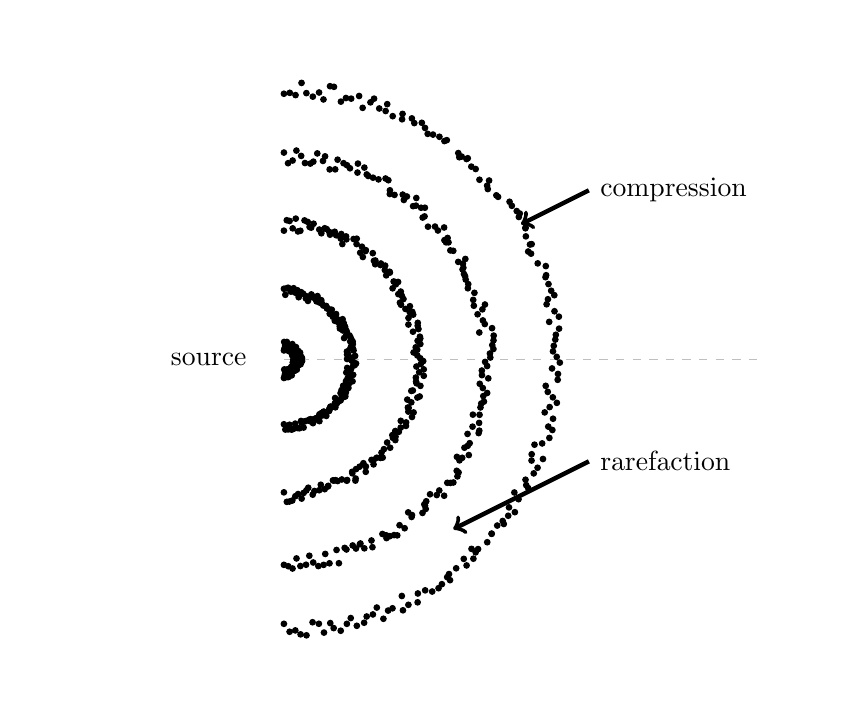
\begin{tikzpicture}
\begin{axis}[height=10cm,
  cycle list={
    only marks,mark size=1pt\\
    only marks,mark size=1pt\\
  },
  % xmin=0,xmax=1.2,
  % ymin=-1,ymax=1,
  domain=270:360+90,
  samples=150,
  axis equal,
  axis line style={draw=none},
  ticks=none,
]
\draw[lightgray,dashed] (0,0) -- (7,0);
\addplot ({(0.2+0.07*rand)*cos(x)},{(0.2+0.07*rand)*sin(x)});
\addplot ({(1.0+0.07*rand)*cos(x)},{(1.0+0.07*rand)*sin(x)});
\addplot ({(2.0+0.10*rand)*cos(x)},{(2.0+0.10*rand)*sin(x)});
\addplot ({(3.0+0.12*rand)*cos(x)},{(3.0+0.12*rand)*sin(x)});
\addplot ({(4.0+0.12*rand)*cos(x)},{(4.0+0.12*rand)*sin(x)});

\draw[<-,ultra thick] (3.5,2) -- ++(axis direction cs: 1,0.5) node[right] {compression};
\draw[<-,ultra thick] (2.5,-2.5) -- ++(axis direction cs: 2,1) node[right] {rarefaction};

\node[left=1em] at (0,0) {source};

\end{axis}
\end{tikzpicture}
\captionsetup{type=figure,margin=1in}
\captionof{figure}{Visualization of a sound wave propagating through air particles.}
\end{center}
\end{document}